% !TeX spellcheck = de_DE
\documentclass{article}
\usepackage{cite}
\usepackage{amsmath,amssymb,amsfonts}
\usepackage{algorithmic}
\usepackage{graphicx}
\usepackage{float} 
\usepackage{subfigure}
\usepackage{textcomp}
\usepackage{xcolor}
\usepackage{booktabs}
\usepackage{caption}
\usepackage[colorlinks]{hyperref}
\usepackage{fontspec, xunicode, xltxtra}  
\usepackage{import}
\usepackage{ctex}
\usepackage{listings}
\usepackage{fontspec} % 定制字体
\newfontfamily\menlo{Menlo}
\usepackage{xcolor} % 定制颜色
\usepackage{underscore}
\definecolor{mygreen}{rgb}{0,0.6,0}
\definecolor{mygray}{rgb}{0.5,0.5,0.5}
\definecolor{mymauve}{rgb}{0.58,0,0.82}
\lstset{ %
	backgroundcolor=\color{white},      % choose the background color
	basicstyle=\footnotesize\ttfamily,  % size of fonts used for the code
	columns=fullflexible,
	tabsize=4,
	breaklines=true,               % automatic line breaking only at whitespace
	captionpos=b,                  % sets the caption-position to bottom
	commentstyle=\color{mygreen},  % comment style
	escapeinside={\%*}{*)},        % if you want to add LaTeX within your code
	keywordstyle=\color{blue},     % keyword style
	stringstyle=\color{mymauve}\ttfamily,  % string literal style
	frame=single,
	rulesepcolor=\color{red!20!green!20!blue!20},
	% identifierstyle=\color{red},
	language=matlab,
}
\usepackage{geometry}
\geometry{a4paper, scale=0.8}
\title{Lab1实验报告}
\author{李文彬,1120173001}
\date{\today}

\begin{document}
	\maketitle
	\section{实验内容}
实验报告中记录了根据实验指导进行实现的操作过程,展示实验各关键部分的截图,绘制要求图表,并在相应阶段回答问题。
\subsection{实验环境}
Macbook pro, macOS Catalina\\Wireshark for Mac

\section{实验流程}
\subsection{Step 1 : Capture a trace}
   \begin{itemize}
\item[1.]打开Wireshark,根据实验指导,在Wireshark中filter栏输入“icmp”
\item[2.]打开Terminal,在终端中输入ping "www.baidu.com" 进行抓包
\item[3.]按“control+c”快捷键停止Terminal中的抓包
   \end{itemize}
   	\subsubsection{过程分析}
   实验过程中,在Terminal中运行ping www.baidu.com 命令,结果如下
   
%	\begin{lstlisting}
%{ % https://ww2.mathworks.cn/help/images/ref/projective2d.html
%
%Origin = imread('~/Downloads/StarZhou.jpeg'); 
%
%
%theta = 10;
%
%tm = [cosd(theta) -sind(theta) 0.0001;
%      sind(theta) cosd(theta) 0.0005;
%      0 0 1];
%
%tform = projective2d(tm);
%
%outputImage = imwarp(Origin, tform);
%
%figure
%subplot(1,2,1),imshow(uint8(Origin)),title('Origin Image')
%subplot(1,2,2),imshow(uint8(outputImage)),title('Perspective Output')
%    \end{lstlisting}
    
   \begin{figure}[H]
        \centering
        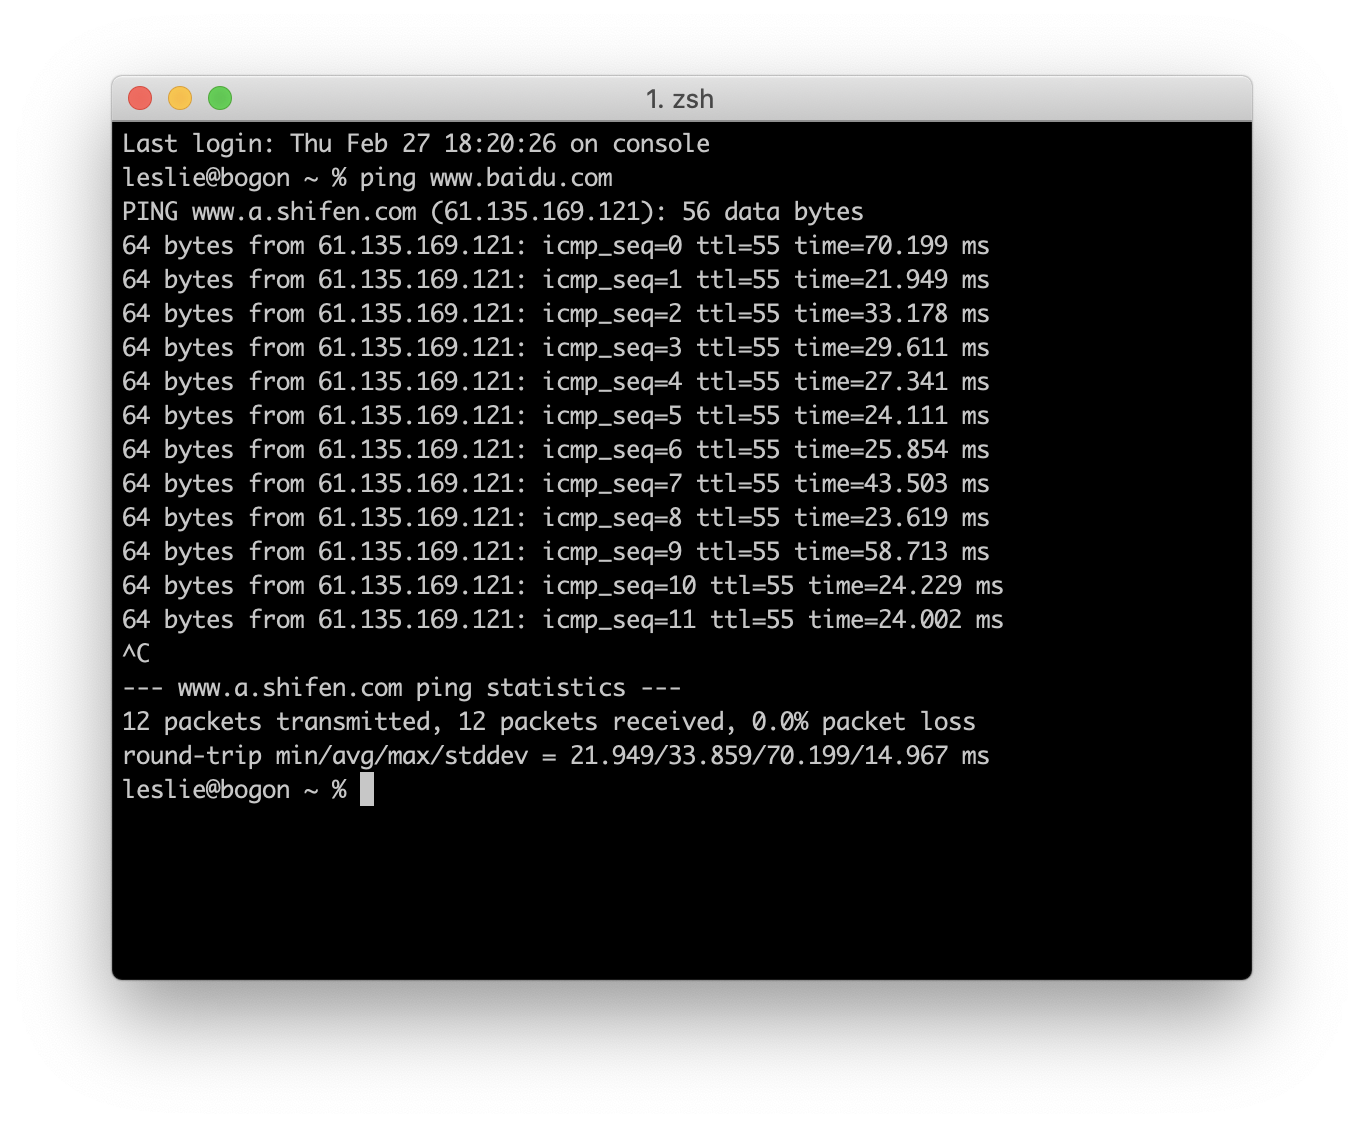
\includegraphics[width=0.9\textwidth]{img/exp12.png}
        \caption{}
        \label{fig.1}
    \end{figure}
    通过wireshark软件捕获ping命令后发送接收的包,结果显示如下:
    \begin{figure}[H]
        \centering
        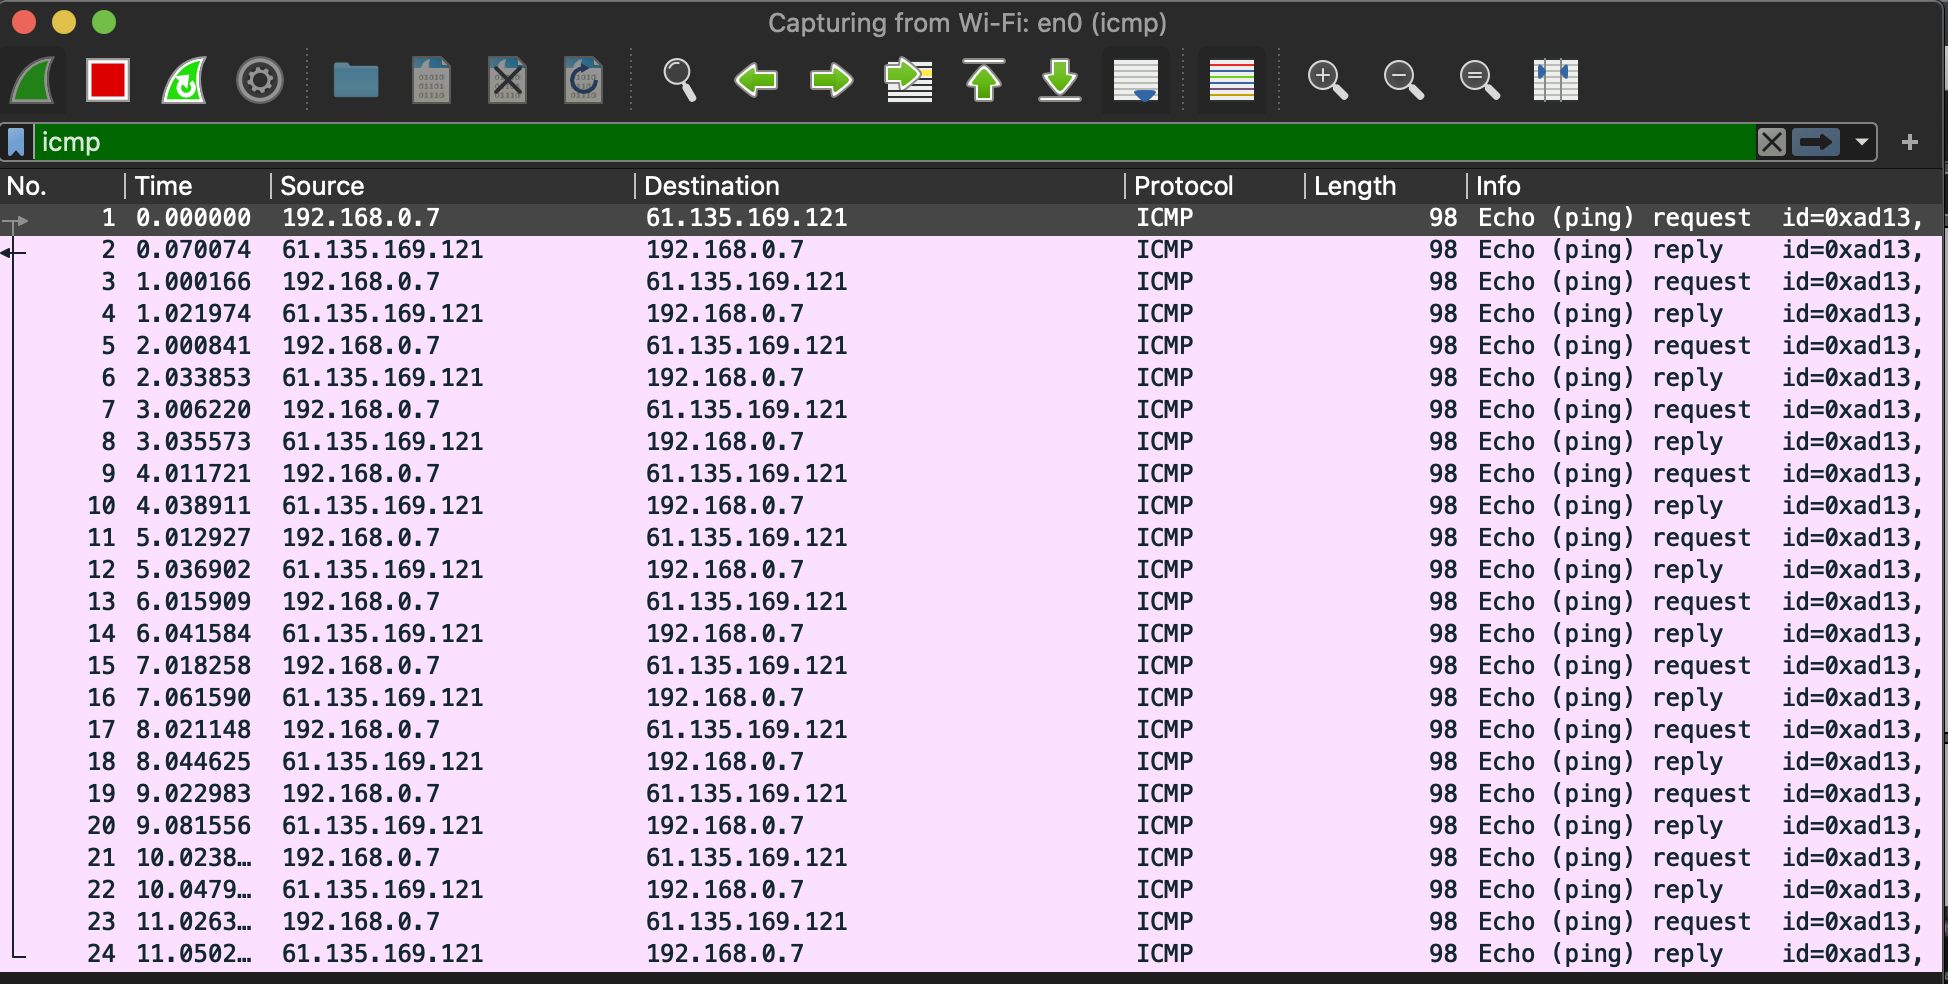
\includegraphics[width=0.9\textwidth]{img/exp1.png}
        \caption{}
        \label{fig.2}
    \end{figure}
  
   
    \subsection{Step 2 : Ethernet Frame Structure}
   随机选取图 2 中的一帧,得到wireshark的自动进行解析,显示如下:
   
  \begin{figure}[H]
        \centering
        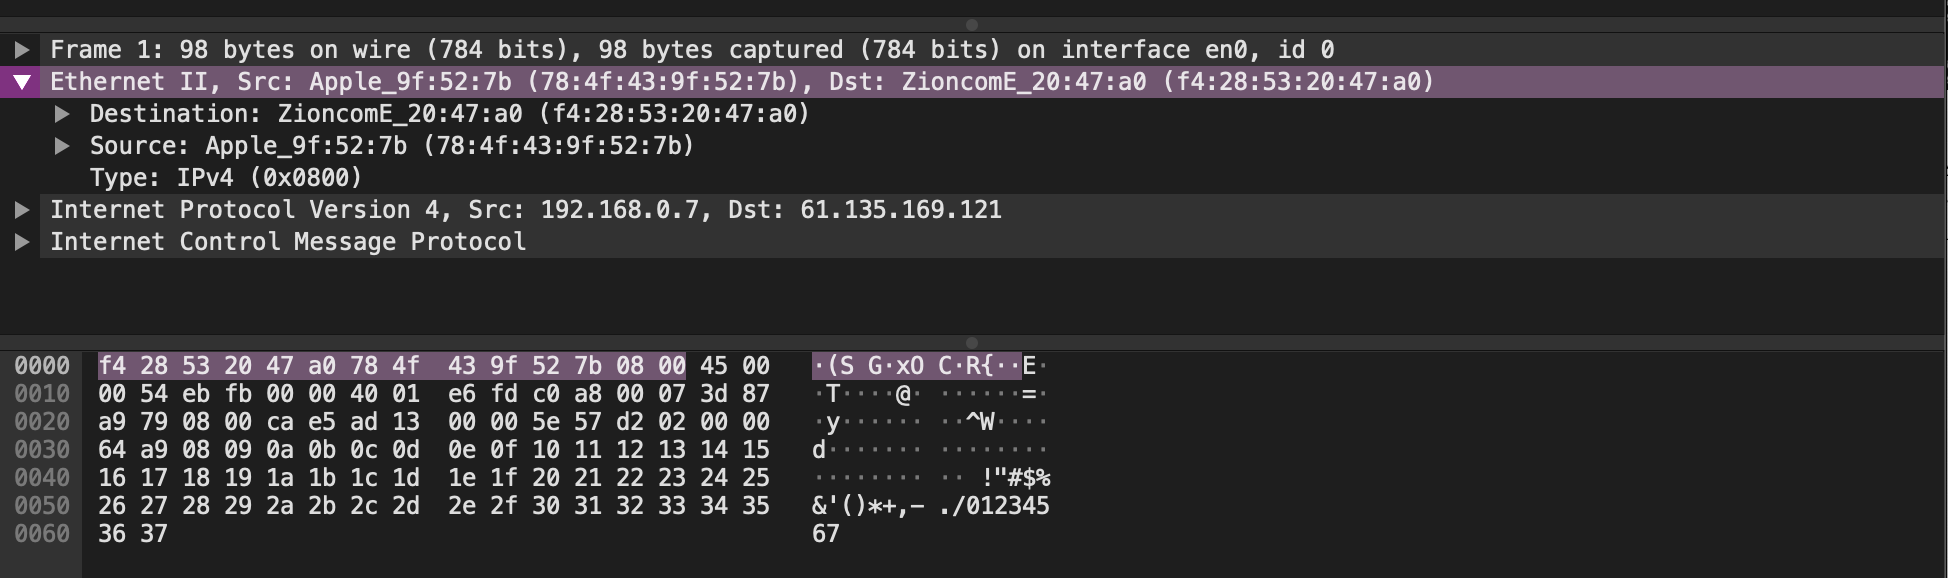
\includegraphics[width=0.9\textwidth]{img/exp123.png}
        \caption{}
        \label{fig.3}
    \end{figure}
  下部显示的信息共0x62字节,与描述98bytes匹配(未计算尾部checksum)。图 3 中选中展开Ethernet部分,Wireshark自动显示其header占14字节。
  
  \subsubsection{Results}
  根据描述信息可知,实验中采用的是Ethernet II协议,由header、data和checksum组成,Ethernet II协议的帧结构如下图:
   \begin{figure}[H]
        \centering
        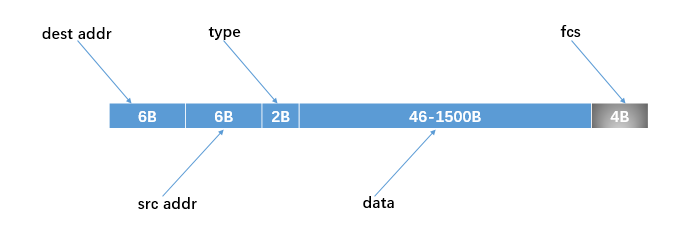
\includegraphics[width=0.9\textwidth]{img/exp123A.png}
        \caption{}
        \label{fig.4}
    \end{figure}
    
    \subsection{Step 3 : Scope of Ethernet Addresses}
    
      \begin{figure}[H]
        \centering
        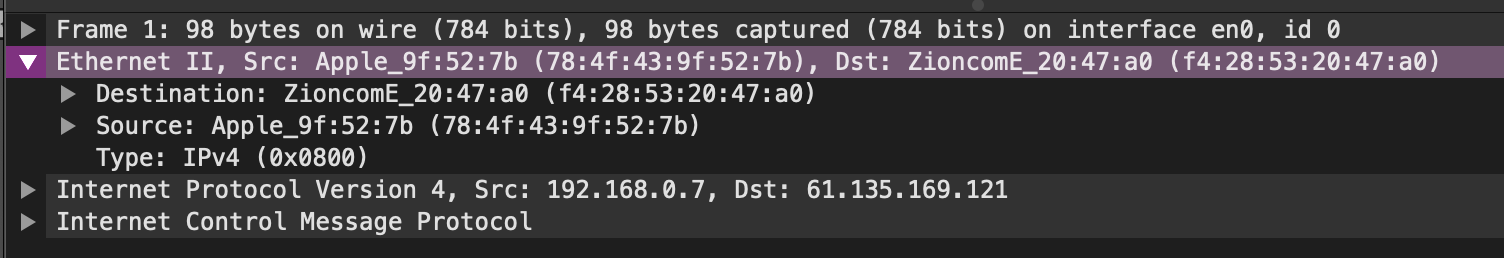
\includegraphics[width=0.9\textwidth]{img/exp123B.png}
        \caption{}
        \label{fig.4}
    \end{figure}
    以上图的Ethernet frame为例,src与dest的物理地址分别为(78:4f:43:9f:52:7b)(18:31:bf:4a:be:80),本机ip为(192.168.0.7),remote server的ip为(61.135.169.121)。因此my computer,router和remote server的相对位置如图所示:
 

    \begin{figure}[H]
        \centering
        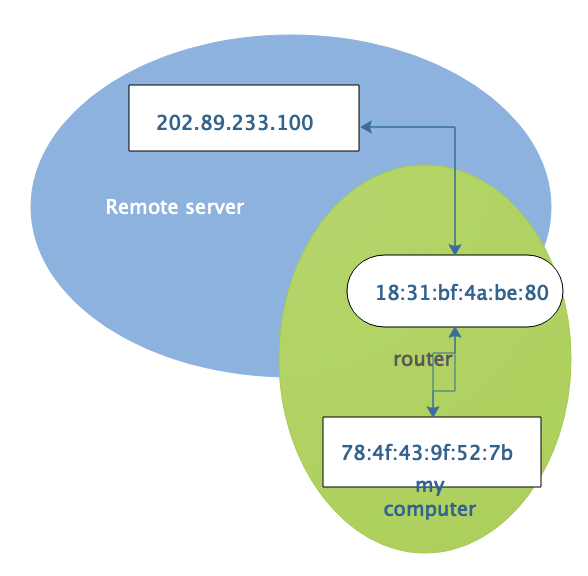
\includegraphics[width=0.6\textwidth]{img/exp123C.png} 
        \caption{}
        \label{fig.5}
    \end{figure}
    
    \section{Broadcast Frames}
    通过如下所示filter,只显示以太网的多播multicast或广播broadcast消息。
    

 \begin{figure}[H]
        \centering
        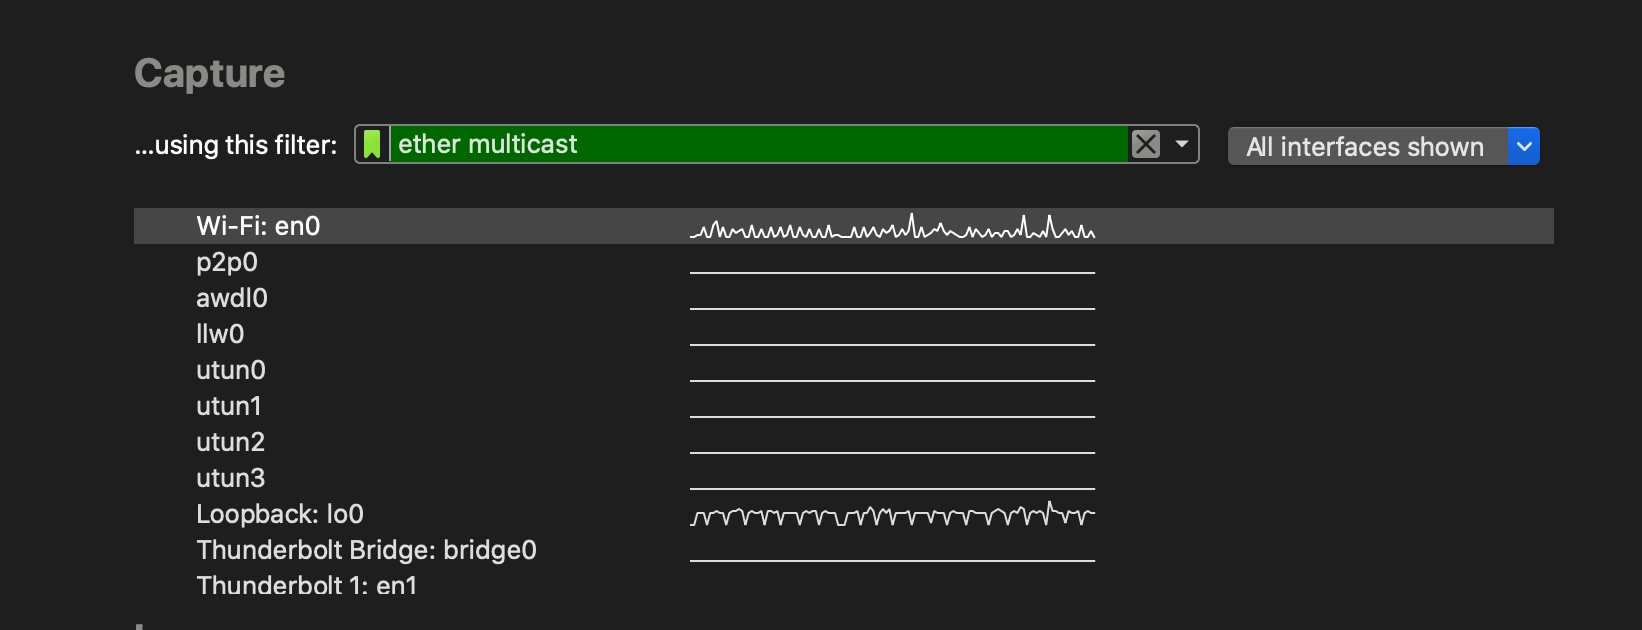
\includegraphics[width=0.9\textwidth]{img/exp1cast.png}
        \caption{}
        \label{fig.6}
    \end{figure}
    以下是截获到的broadcast和multicast样例。
     \begin{figure}[H]
        \centering
        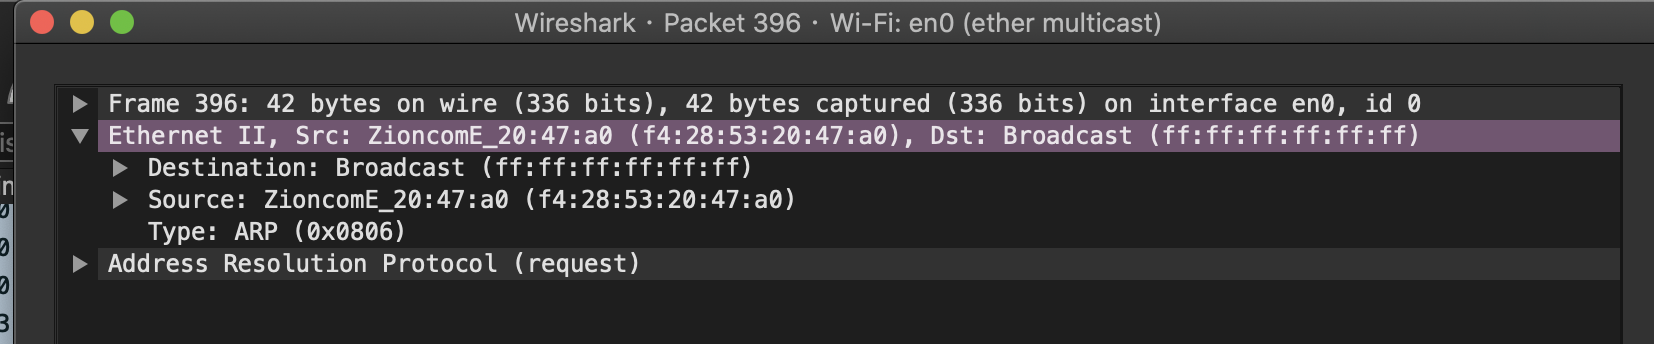
\includegraphics[width=0.9\textwidth]{img/exp1broad.png}
        \caption{}
        \label{fig.7}
    \end{figure}
    \begin{figure}[H]
        \centering
        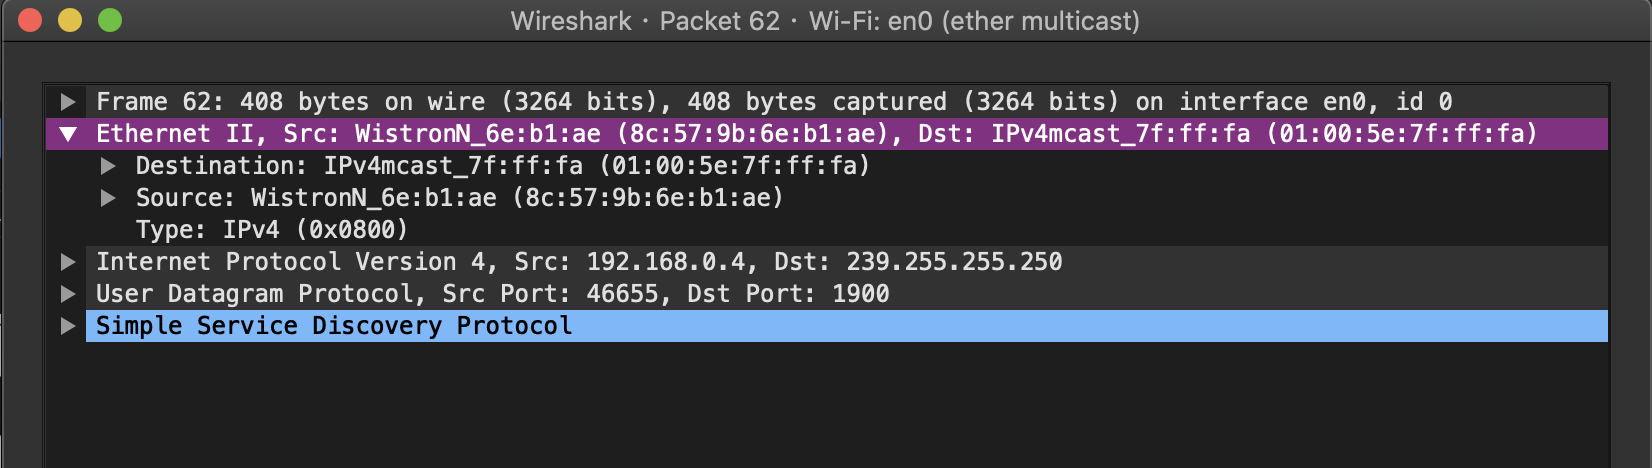
\includegraphics[width=0.9\textwidth]{img/exp1multi.png}
        \caption{}
        \label{fig.8}
    \end{figure}
  
\section{Answering the following question}
 \begin{itemize}
 \item[i]What is the broadcast Ethernet address, written in standard form as Wireshark displays it?
 \item[]图8可见,broadcast的目的地址为(ff:ff:ff:ff:ff:ff),即48bit全为1。
 \item[ii]whether it is unicast or multicast/broadcast?
 \item[]分析multicast的目的物理地址段,wireshark软件显示Group address标志位为第8位,如下图所示,其地址的第一字节为01H,标识位为1表示多播。
 \end{itemize}
  \begin{figure}[H]
        \centering
        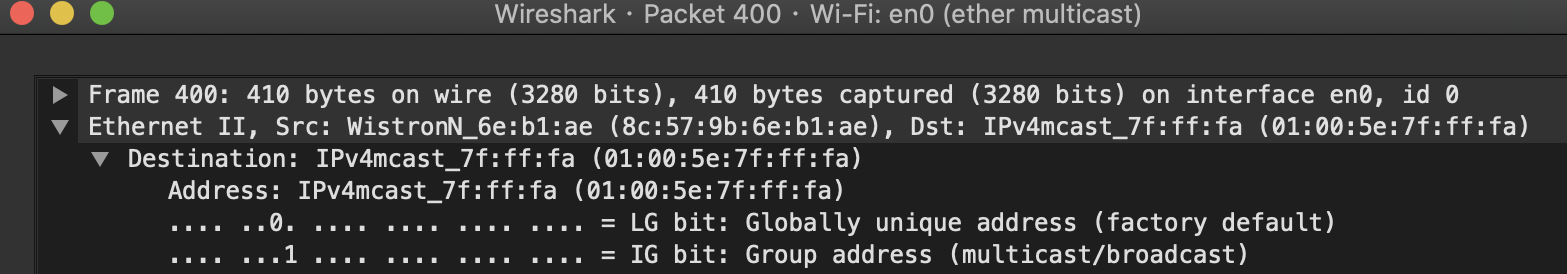
\includegraphics[width=0.9\textwidth]{img/exp1multi1.png}
        \caption{}
        \label{fig.9}
    \end{figure}



 
\end{document}